\documentclass[report.tex]{subfiles}
\graphicspath{ \subfix{./images/} \subfix{./graphs/} }
\begin{document}
\section{Milestone 6: Handle API calls}

By following the instructions of the Microsoft Graph API documentation\cite{microsoft:docs:education-overview}, I login the Graph Explorer\cite{microsoft:graph-explorer} and run a \code{GET} query over the \code{/education/schools} endpoint. However, I received a 400 bad request.

\begin{minted}{json}
{
    "error": {
        "code": "Request_UnsupportedQuery",
        "message": "Property 'extension_fe2174665583431c953114ff7268b7b3_Education_ObjectType' does not exist as a declared property or extension property.",
        "innerError": {
            "date": "2022-03-16T23:57:05",
            "request-id": "1bc8bdfa-ee27-48fd-9e89-7d2a3c5352f6",
            "client-request-id": "76d647a4-e41c-7da1-02e6-77bd39398e72"
        }
    }
}
\end{minted}

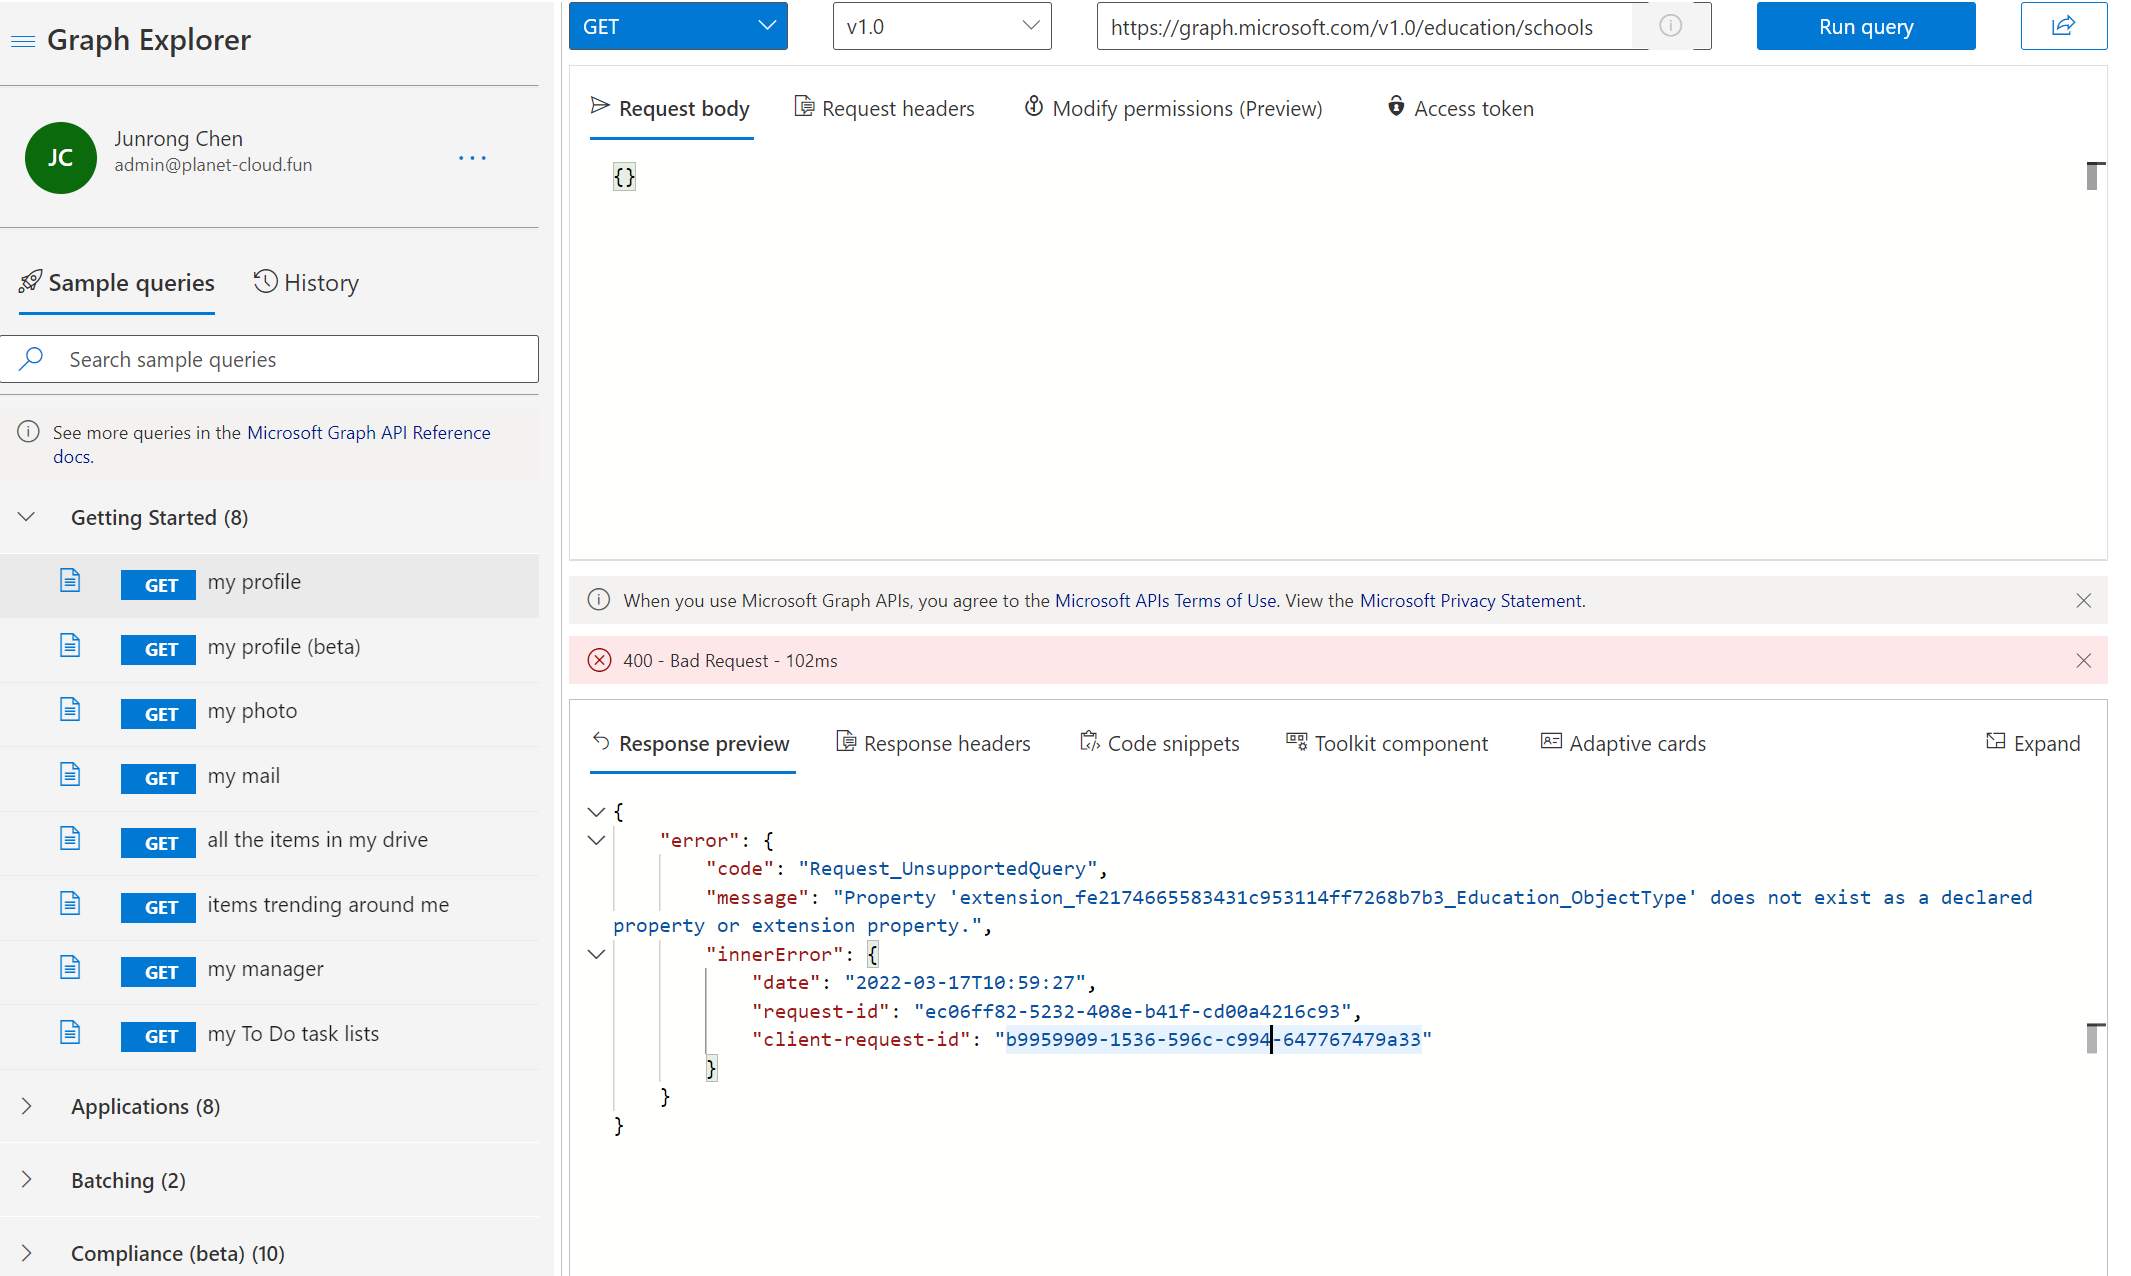
\includegraphics[width=\textwidth, height=\textheight, keepaspectratio]{GraphExplorerBadRequest}

After some investigation, I must have an admin account of an education organization to call these education APIs.

I then tried my school account, which belongs to an educational organization.

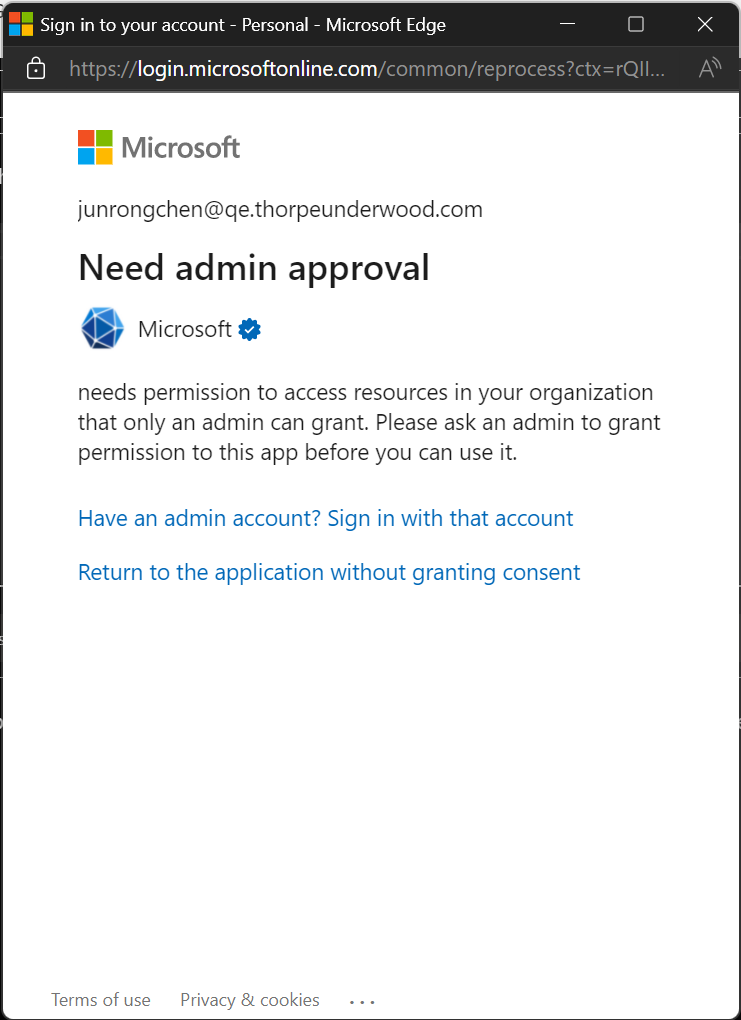
\includegraphics[width=\textwidth, height=\textheight, keepaspectratio]{EducationAPINeedApproval}

But unfortunately, my student account is not an admin and therefore has no permission to call these APIs as well.

Considering that I can't register as an education organization, and I can't ask for an admin account from my school, the integration with Microsoft Teams for Education is not possible to implement.

Even if I can use these API, the Judging security issue which I mentioned before still applies. Therefore I decided not to implement this part of the project. All of my stakeholders express that they understand this limitation and they agree with my decision.

\end{document}